% %% file: template.tex = LaTeX template for article-like report 
%% init: sometime 1993
%% last: Feb  8 2015  Rob Rutten  Deil
%% site: http://www.staff.science.uu.nl/~rutte101/rrweb/rjr-edu/manuals/student-report/

%% First read ``latex-bibtex-simple-manual.txt'' at
%% http://www.staff.science.uu.nl/~rutte101/Report_recipe.html

%% Start your report production by copying this file into your XXXX.tex.
%% Small changes to the header part will make it an A&A or ApJ manuscript.

%%%%%%%%%%%%%%%%%%%%%%%%%%%%%%%%%%%%%%%%%%%%%%%%%%%%%%%%%%%%%%%%%%%%%%%%%%%%
\documentclass{aa}   %% Astronomy & Astrophysics style class
%\documentclass[a4paper,10pt]{report}
\usepackage{graphicx,url,twoopt}
%\usepackage{biblatex}
\usepackage{enumitem}
\usepackage{amsmath}
\usepackage[varg]{txfonts}           %% A&A font choice
%\usepackage{hyperref}                %% for pdflatex
%%\usepackage[breaklinks]{hyperref}  %% for latex+dvips
%%\usepackage{breakurl}              %% for latex+dvips
%\usepackage{pdfcomment}              %% for popup acronym meanings
%\usepackage{acronym}                 %% for popup acronym meanings
\usepackage{calrsfs}
\DeclareMathAlphabet{\pazocal}{OMS}{zplm}{m}{n}

\usepackage{natbib}
% \hypersetup{
%   colorlinks=true,   %% links colored instead of frames
%   urlcolor=blue,     %% external hyperlinks
%   linkcolor=red,     %% internal latex links (eg Fig)
% }

 %\bibpunct{(}{)}{;}{a}{}{,}    %% natbib cite format used by A&A and ApJ
 
 \pagestyle{plain}   %% undo the fancy A&A pagestyle 

%% Add commands to add a note or link to a reference
\makeatletter
\newcommand{\bibnote}[2]{\@namedef{#1note}{#2}}
\newcommand{\biblink}[2]{\@namedef{#1link}{#2}}
\makeatother

%% Commands to make citations ADS clickers and to add such also to refs
%% May 2014: they give error stops ("Illegal parameter number ..."}
%%   for plain latex with TeX Live 2013; the ad-hoc fixes added below let
%%   latex continue instead of stop within these commands.
%%   Please let me know if you know a better fix!
%%   No such problem when using pdflatex.
\makeatletter
 \newcommandtwoopt{\citeads}[3][][]{%
   \nonstopmode%              %% fix to not stop at error message in latex
   \href{http://adsabs.harvard.edu/abs/#3}%
        {\def\hyper@linkstart##1##2{}%
         \let\hyper@linkend\@empty\citealp[#1][#2]{#3}}%   %% Rutten, 2000
   \biblink{#3}{\href{http://adsabs.harvard.edu/abs/#3}{ADS}}%
   \errorstopmode}            %% fix to resume stopping at error messages 
 \newcommandtwoopt{\citepads}[3][][]{%
   \nonstopmode%              %% fix to not stop at error message in latex
   \href{http://adsabs.harvard.edu/abs/#3}%
        {\def\hyper@linkstart##1##2{}%
         \let\hyper@linkend\@empty\citep[#1][#2]{#3}}%     %% (Rutten 2000)
   \biblink{#3}{\href{http://adsabs.harvard.edu/abs/#3}{ADS}}%
   \errorstopmode}            %% fix to resume stopping at error messages
 \newcommandtwoopt{\citetads}[3][][]{%
   \nonstopmode%              %% fix to not stop at error message in latex
   \href{http://adsabs.harvard.edu/abs/#3}%
        {\def\hyper@linkstart##1##2{}%
         \let\hyper@linkend\@empty\citet[#1][#2]{#3}}%     %% Rutten (2000)
   \biblink{#3}{\href{http://adsabs.harvard.edu/abs/#3}{ADS}}%
   \errorstopmode}            %% fix to resume stopping at error messages 
 \newcommandtwoopt{\citeyearads}[3][][]{%
   \nonstopmode%              %% fix to not stop at error message in latex
   \href{http://adsabs.harvard.edu/abs/#3}%
        {\def\hyper@linkstart##1##2{}%
         \let\hyper@linkend\@empty\citeyear[#1][#2]{#3}}%  %% 2000
   \biblink{#3}{\href{http://adsabs.harvard.edu/abs/#3}{ADS}}%
   \errorstopmode}            %% fix to resume stopping at error messages 
\makeatother

%%%%%%%%%%%%%%%%%%%%%%%%%%%%%%%%%%%%%%%%%%%%%%%%%%%%%%%%%%%%%%%%%%%%%%%%%%%%
\begin{document}  

%% simple header.  Change into A&A or ApJ commands for those journals

\twocolumn[{%
\vspace*{4ex}

\begin{center}
  {\Large \bf The background evolution of the universe}\\[4ex]
  {\large \bf Andreas Ellewsen$^1$}\\[4ex]
  \begin{minipage}[t]{15cm}
        $^1$ Institute of Theoretical Astrophysics, University of Oslo, P.O. Box 1029 Blindern, N-0315 Oslo, Norway\\
             
        
    {\bf Abstract.} I set up the background cosmology of the universe.
    
  \vspace*{2ex}
  \end{minipage}
\end{center}
}]

%%%%%%%%%%%%%%%%%%%%%%%%%%%%%%%%%%%%%%%%%%%%%%%%%%%%%%%%%%%%%%%%%%%%%%%%%%%%
\section{Introduction}\label{sec:introduction}
%%%%%%%%%%%%%%%%%%%%%%%%%%%%%%%%%%%%%%%%%%%%%%%%%%%%%%%%%%%%%%%%%%%%%%%%%%%%
In this project I will follow the algorithm presented in Callin (2005)[1] for simulating the cosmic microwave background.  
This is part one of four for this project.
The first part involves computing the expansion history of the universe, as well as looking at the evolution of the density of various matter and energy components. This sets up the background cosmology such that we in the next step can turn to perturbations.
I have chosen to make this first part compatible with the inclusion of neutrinos.
This can of course be removed by setting the neutrino density to zero and raising the radiation density accordingly.

To ease the development of this code, I have been provided with a skeleton code of the project. 
This code includes a variety of methods needed to solve the project. These methods will be explained as they are used throughout the  project.

%%%%%%%%%%%%%%%%%%%%%%%%%%%%%%%%%%%%%%%%%%%%%%%%%%%%%%%%%%%%%%%%%%%%%%%%%%%%
\section{Equations}\label{sec:Equations}
%%%%%%%%%%%%%%%%%%%%%%%%%%%%%%%%%%%%%%%%%%%%%%%%%%%%%%%%%%%%%%%%%%%%%%%%%%%%
For the background cosmology I use the standard Friedmann-Lemaître-Robertson-Walker(FLRW) metric for flat space.
This gives the line element.
\begin{equation}\label{FLRW}
\begin{aligned}
ds^2 &= -dt^2 +a^2(t)(r^2(d\theta^2+sin^2\theta d\phi^2)\\
     &=a^2(\eta)(-d\eta^2 +r^2(d\theta^2+sin^2\theta d\phi^2))
\end{aligned}
\end{equation}
where $a(t)$ is the scale factor, and $\eta$ conformal time.
I also introduce a parameter $x$ defined as 
\begin{equation}\label{xeq}
 x = ln(a)
\end{equation}
The redshift is defined as
\begin{equation}
 1+ z =\frac{a_0}{a}
\end{equation}

We assume that the universe consist of cold dark matter (CDM, m), baryons (b), radiation(r), neutrinos($\nu$), and a cosmological constant ($\Lambda$). 
With these components, the Hubble parameter $H$ becomes
\begin{equation}
 H = \frac{1}{a}\frac{da}{dt} = H_0\sqrt{(\Omega_m+\Omega_b)a^{-3}+(\Omega_r+\Omega_\nu)a^{-4}+\Omega_\Lambda}.
\end{equation}
I also introduce a scaled $H$, namely
\begin{equation}
\begin{aligned}
\pazocal{H} &= \frac{1}{a}\frac{da}{d\eta} \equiv \frac{\dot{a}}{a} = aH\\
&=H_0\sqrt{(\Omega_m+\Omega_b)a^{-1}+(\Omega_r+\Omega_\nu)a^{-2}+\Omega_\Lambda a^2}.
\end{aligned}
\end{equation}
Note that the dot means derivative with respect to conformal time. Why this is useful will become apparent later.
We also want the derivative of this with respect to $x$.

\begin{equation}
 \frac{d\pazocal{H}}{dx} = H_0\frac{-(\Omega_m+\Omega_b)e^{-x}-2(\Omega_r+\Omega_\nu)e^{-2x}+2\Omega_\Lambda e^{2x}}{\sqrt{(\Omega_m+\Omega_b)e^{-x}+(\Omega_r+\Omega_\nu)e^{-2x}+\Omega_\Lambda e^{2x}}}.
\end{equation}

$\Omega_x$ is the relative density of component x compared to the critical density $\rho_c$ needed for the universe to be flat.
\begin{equation}
 \Omega_x = \frac{\rho_x}{\rho_c}
\end{equation}
\begin{equation}
 \rho_c = \frac{3H^2}{8\pi G}
\end{equation}
We want to keep track of the densities of each component.
\begin{equation}
 \rho_m = \rho_{m,0}a^{-3}
\end{equation}
\begin{equation}
 \rho_b = \rho_{b,0}a^{-3}
\end{equation}
\begin{equation}
 \rho_r = \rho_{r,0}a^{-4}
\end{equation}
\begin{equation}
 \rho_\nu = \rho_{\nu,0}a^{-4}
\end{equation}
\begin{equation}
 \rho_\Lambda = \rho_{\Lambda,0}
\end{equation}

We will also need to know the distance to the particle horizon at different times. This can be found by noting that
\begin{equation*}
 \frac{d\eta}{dt} = \frac{c}{a}
\end{equation*}
which can be rewritten such that
\begin{equation}\label{eta}
 \frac{d\eta}{da} = \frac{c}{a \pazocal{H}}
\end{equation}
There are two ways to solve this differential equation numerically. One can either intergrate directly, or one can use an ordinary differential equation solver(ODE solver). Since the skeleton code contains an ODE solver I have chosen the latter. (See section \ref{sec:Imp} for more information).

%%%%%%%%%%%%%%%%%%%%%%%%%%%%%%%%%%%%%%%%%%%%%%%%%%%%%%%%%%%%%%%%%%%%%%%%%%%%
\section{Implementation}\label{sec:Imp}
%%%%%%%%%%%%%%%%%%%%%%%%%%%%%%%%%%%%%%%%%%%%%%%%%%%%%%%%%%%%%%%%%%%%%%%%%%%%
The programming language of choice is Fortran90. This is chosen because of its speed, and because the skeleton code provided was written in it. 

The first step is to set up arrays for $a$, $x$, $\eta$, all five $\Omega_x$, and $\rho_x$. We will also need arrays for $\rho_c$, $H$, and $z$.

We then set the first $x$ value to correspond to $a= 10^{-10}$, and the last to $a=0$ (today). 
I've chosen to use 1000 points for these arrays and make the steps equal in the $x$ array. After that one computes the $a$, and $z$ values for each of the points in this $x$ array. Because of this we now have linear steps in $x$.
With that done, one computes $H$, $\pazocal{H}$, $\rho_x$, and $\Omega_x$ for each $x$ value.

The last thing to find is $\eta(x)$. 
To do this we need to use an ODE solver on equation \ref{eta}. For this we must have some initial value for the function. 
The equation we then want to solve is 
\begin{equation}
 \eta(a) = \int_0^a \frac{da'}{a'\pazocal{H}(a')}
\end{equation}

This can be found by considering that $a\pazocal{H} \rightarrow  H_0\sqrt{\Omega_r+\Omega_\nu}$ as $a \rightarrow 0$. This gives 
\begin{equation}
 \eta(a) = \frac{a}{H_0\sqrt{\Omega_r+\Omega_\nu}}
\end{equation}
for small $a$. And thus one has an initial value.

Plugging this into the ODE solver returns $\eta(x)$ for all values in the $x$ array. Thus completing all calculations needed for the first part of the project. The ODE solver uses the Bulirsch–Stoer algorithm. The steplength is set to be one hundredth the length between two neighbouring $x$ values.

As preparation for the next part I also spline the resulting $\eta(x)$ values. These are then integrated and evaluated for a new set of $x$ values not equal to but inside the $x$ values used to make the spline. I have overplotted this in the plot for $\eta(x)$ and the functions overlap. 

%%%%%%%%%%%%%%%%%%%%%%%%%%%%%%%%%%%%%%%%%%%%%%%%%%%%%%%%%%%%%%%%%%%%%%%%%%%%
\section{Results}\label{sec:simulate_analytic}
%%%%%%%%%%%%%%%%%%%%%%%%%%%%%%%%%%%%%%%%%%%%%%%%%%%%%%%%%%%%%%%%%%%%%%%%%%%%
 The $\Omega_x$ values indicate the relative density of a given component compared to the critical density of the universe. 
 The critical density being that which corresponds to the universe begin flat.
 Looking at the figure we see radiation dominating from the start together with neutrinos.
 This continues for some time until the dark matter component starts to rise.
 We see that this starts before the baryon component. This is good since that makes it possible for dark matter to form structures that baryons can later fall into. The radiation and neutrinos die out, and at a later point vacuum energy shoots up. At the end we end up with approximately 70\% vacuum energy(dark energy?), 25\% dark matter, and 5\% baryons. This is exactly as it should be since that is what they were set to be at the present. See figure \ref{figure0}.
 \begin{figure}[ht]
  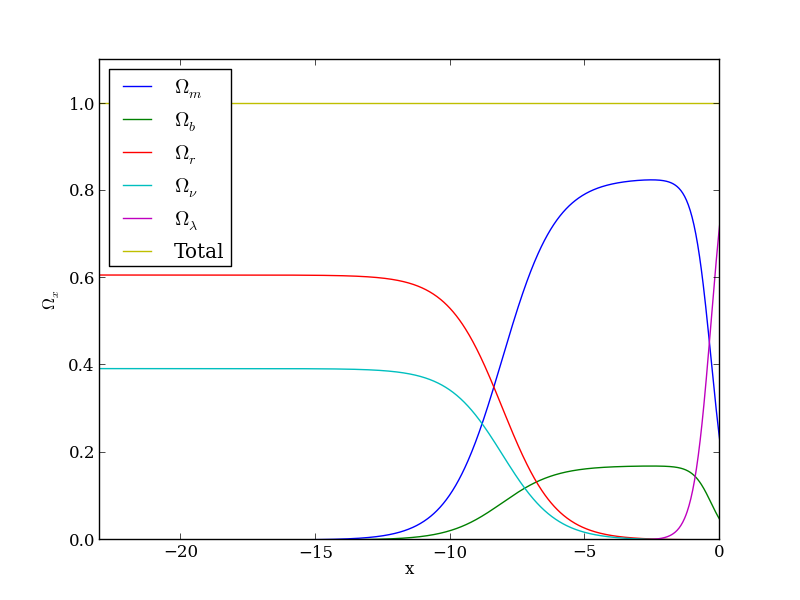
\includegraphics[width=.49\textwidth]{figure_0.png}
  \caption{The figure shows the evolution of the relative densities. As described they behave as they should.}
 \label{figure0}
 \end{figure}
 
 Conformal time, denoted $\eta(x)$ measures the distance to the particle horizon for a given $x$ value. A nice test of this is to insert the $x$ value of today.
 The answer should then be the radius of the observable universe. At the present this is measured to be approximately 14 billion parsecs (14Gpc)[2]
 The graph hits this value fairly well, indicating that everything is working properly so far. 
 Note also that there are in fact two graphs in this figure, one which is calculated from the differential equation for $\eta$. 
 And another one made by splining the first one and finding $\eta$ values at arbitrary values between those of the first function.
 
  \begin{figure}[ht]
  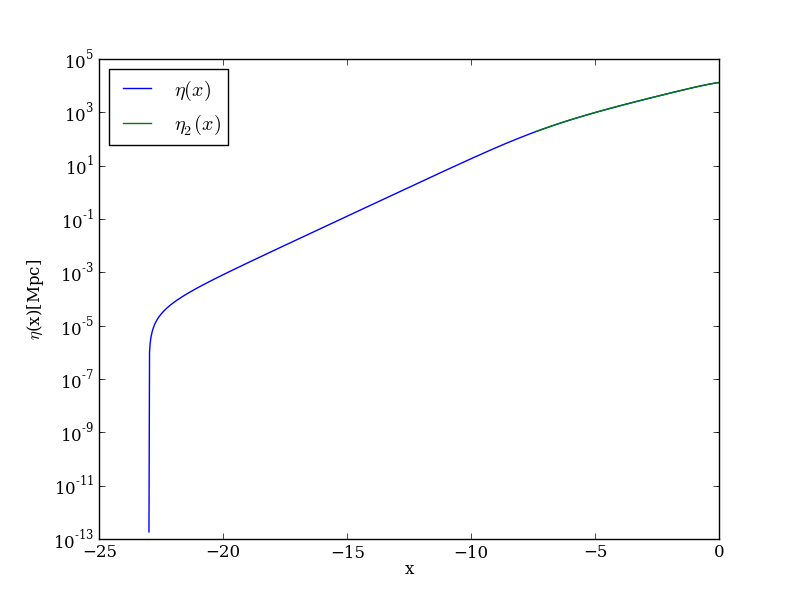
\includegraphics[width=.49\textwidth]{figure_1.png}
  \caption{The conformal time hits the value of today fairly accurately. The splined function hits the computed values so well that they overlap. Here $\eta(x)$ is the computed function, while $\eta_2(x)$ is the splined one.}
 \label{figure1}
 \end{figure}
 
 The Hubble parameter $H$ is depicted both as a function of $x$, and $z$. Whether this is good or not is hard to say for the first part. We can at least put some faith in its precision by the fact that it ends at $H_0 \approx 70$km s$^{-1}$Mpc$^{-1}$, which is what $H_0$ was set to be. 
 
  \begin{figure}[ht]
  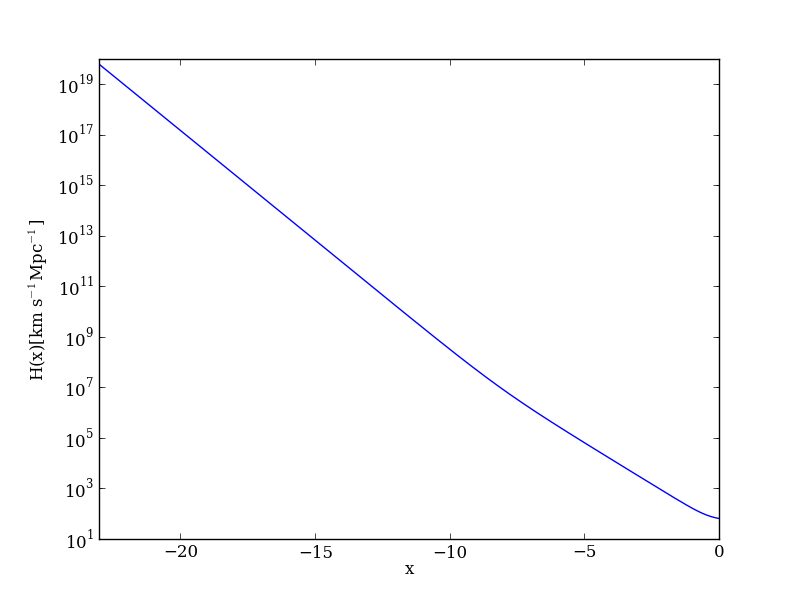
\includegraphics[width=.49\textwidth]{figure_2.png}
  \caption{The figure depicts the Hubble parameter as a function of $x$.}
 \label{figure2}
 \end{figure}
 
 \begin{figure}[ht]
  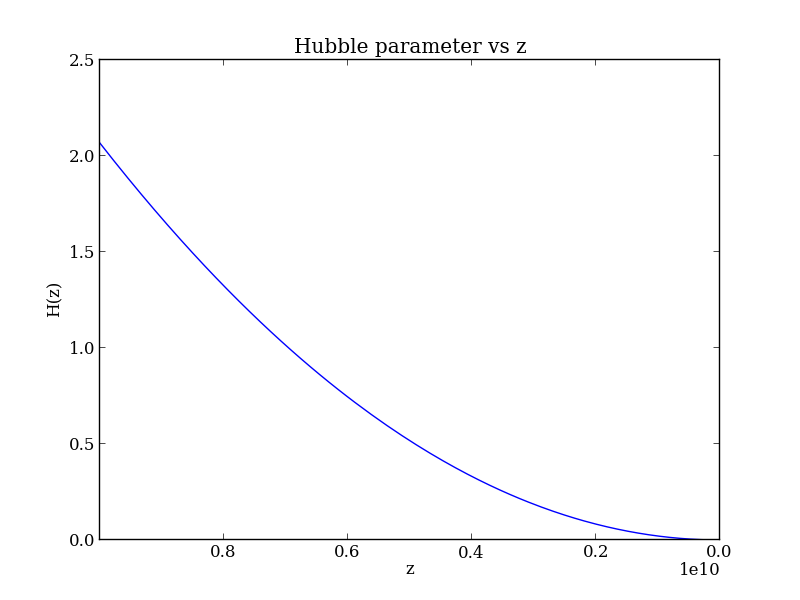
\includegraphics[width=.49\textwidth]{figure_3.png}
  \caption{The figure depcits the Hubble parameter as a function of redshift $z$. Note that $z$ increases to the left, such that time goes towards the right.}
 \label{figure3}
 \end{figure}
% 
% \begin{table}
%  \begin{tabular}{|c|c|c|}
%   \hline
%   &Analytical &Numerical \\
%   \hline
%   $<E>$ &-1.996 & -1.996\\
%   \hline
%   $<|M|>$& 0.999& 0.999\\
%   \hline
%   $C_V$ & 0.032& 0.032\\
%   \hline
%   $\chi$ & 0.004& 0.004\\
%   \hline
%  \end{tabular}
% \caption{Table of values from the analytical calculations for a system with L=2 and T = 1 in units of (kT/J). Note the precision of the numerical result.}
% \label{tab1}
% \end{table}

%%%%%%%%%%%%%%%%%%%%%%%%%%%%%%%%%%%%%%%%%%%%%%%%%%%%%%%%%%%%%%%%%%%%%%%%%%%%
\section{Conclusions} \label{sec:conclusions}
%%%%%%%%%%%%%%%%%%%%%%%%%%%%%%%%%%%%%%%%%%%%%%%%%%%%%%%%%%%%%%%%%%%%%%%%%%%%
The background cosmology of the universe is done and everything has worked the way it was expected to.
There are some values that I do not have an intuition for what should be. Namely the Hubble parameter at times before today. However, I expect these to be correct since everything else has given results generally considered to be correct, and the Hubble parameter is computed directly from these values.
With this, the code is ready for the introduction of perturbations in part two. 

%%%%%%%%%%%%%%%%%%%%%%%%%%%%%%%%%%%%%%%%%%%%%%%%%%%%%%%%%%%%%%%%%%%%%%%%%%%%
\section{References}
%%%%%%%%%%%%%%%%%%%%%%%%%%%%%%%%%%%%%%%%%%%%%%%%%%%%%%%%%%%%%%%%%%%%%%%%%%%%
\begin{enumerate}[label= {[}\arabic*{]} ]
 \item P. Callin, astro-ph/0606683
 \item I. Bars and J. Terning, Extra Dimensions in Space and Time, Springer 2010
\end{enumerate}



%\bibliographystyle{aa-note} %% aa.bst but adding links and notes to references
%\raggedright              %% only for adsaa with dvips, not for pdflatex
%\bibliographystyle{unsrt}
%\bibliography{bibliography}{}       %% XXX.bib = your Bibtex entries copied from ADS

\onecolumn 
%%%%%%%%%%%%%%%%%%%%%%%%%%%%%%%%%%%%%%%%%%%%%%%%%%%%%%%%%%%%%%%%%%%%%%%%%%%%
\section{Source code}\label{sec:files}
%%%%%%%%%%%%%%%%%%%%%%%%%%%%%%%%%%%%%%%%%%%%%%%%%%%%%%%%%%%%%%%%%%%%%%%%%%%%
The source code for the time\_mod file is included for inspection. Note that the code makes use of several different files, one with various parameters, as well as the ODE solver, and the spline.
\begin{verbatim}
 module time_mod
  use healpix_types
  use params
  use spline_1D_mod
  use ode_solver
  implicit none

  integer(i4b)                           :: n_t                ! Number of x-values
  real(dp),    allocatable, dimension(:) :: x_t                ! Grid of relevant x-values
  real(dp),    allocatable, dimension(:) :: a_t                ! Grid of relevant a-values
  real(dp),    allocatable, dimension(:) :: eta_t              ! Grid of relevant eta-values

  integer(i4b)                           :: n_eta              ! Number of eta grid poins
  real(dp),    allocatable, dimension(:) :: z_eta 		!Grid points for eta
  real(dp),    allocatable, dimension(:) :: x_eta              ! Grid points for eta
  real(dp),    allocatable, dimension(:) :: a_eta              ! Grid points for eta
  real(dp),    allocatable, dimension(:) :: eta, eta2          ! Eta and eta'' at each grid point
  real(dp),    allocatable, dimension(:) :: dydx


  real(dp)    				 :: rho_m0 !matter density today
  real(dp) 				 :: rho_b0 !baryong density today
  real(dp)				 :: rho_r0 !radiation density today
  real(dp) 				 :: rho_nu0 !neutrino density today
  real(dp)				 :: rho_lambda0 !vacuum energy density today

  real(dp),    allocatable, dimension(:) :: rho_m !matter density
  real(dp),    allocatable, dimension(:) :: rho_b !baryong density
  real(dp),    allocatable, dimension(:) :: rho_r !radiation density
  real(dp),    allocatable, dimension(:) :: rho_nu !neutrino density
  real(dp),    allocatable, dimension(:) :: rho_lambda !vacuum energy density

  real(dp),    allocatable, dimension(:) :: Omega_mx !Relative densities
  real(dp),    allocatable, dimension(:) :: Omega_bx
  real(dp),    allocatable, dimension(:) :: Omega_rx 
  real(dp),    allocatable, dimension(:) :: Omega_nux 
  real(dp),    allocatable, dimension(:) :: Omega_lambdax 

  real(dp),    allocatable, dimension(:) :: H !Huble constant as func of x


contains

  subroutine initialize_time_mod
    implicit none

    integer(i4b) :: i, n, n1, n2
    real(dp)     :: z_start_rec, z_end_rec, z_0, x_start_rec, x_end_rec, x_0
    real(dp)     :: dx, x_eta1, x_eta2, a_init,h1,eta_init,a_end,rho_crit0,rho_crit
    real(dp)     :: eps,hmin,yp1,ypn


    ! Define two epochs, 1) during and 2) after recombination.
    n1          = 200                       ! Number of grid points during recombination
    n2          = 300                       ! Number of grid points after recombination
    n_t         = n1 + n2                   ! Total number of grid points

    z_start_rec = 1630.4d0                  ! Redshift of start of recombination
    z_end_rec   = 614.2d0                   ! Redshift of end of recombination
    z_0         = 0.d0                      ! Redshift today

    x_start_rec = -log(1.d0 + z_start_rec)  ! x of start of recombination
    x_end_rec   = -log(1.d0 + z_end_rec)    ! x of end of recombination
    x_0         = 0.d0                      ! x today
    
    n_eta       = 1000                      ! Number of eta grid points (for spline)
    a_init      = 1.d-10                    ! Start value of a for eta evaluation
    a_end       = 1.d0
    x_eta1      = log(a_init)               ! Start value of x for eta evaluation
    x_eta2      = 0.d0                      ! End value of x for eta evaluation
    eta_init    = a_init/(H_0*sqrt(Omega_r+Omega_nu))

    eps = 1.d-10
    hmin = 0.d0

    ! Task: Fill in x and a grids ( These will be used in later milestones)
    allocate(x_t(n_t))

    do i = 0,n1-1 ! Fill interval during recombination
       x_t(i+1)= x_start_rec + i*(x_end_rec-x_start_rec)/(n1-1)
    end do

    do i = 1,n2 !Fill from end of recomb to today
        x_t(n1+i) = x_end_rec + (i)*(x_0-x_end_rec)/(n2)
    end do

    !write(*,*) x_t !print x_t to terminal


    allocate(a_t(n_t+1))
    a_t = exp(x_t) !fill the a grid using the x grid

    !write(*,*) a_t !print a_t to terminal


    !Allocate and fill a,x, and z arrays
    allocate(a_eta(n_eta))
    allocate(x_eta(n_eta))
    allocate(z_eta(n_eta))

    x_eta(1) = x_eta1
    do i = 1,n_eta-1
        x_eta(i+1) = x_eta1 + i*(x_eta2-x_eta1)/(n_eta-1)
    end do

    a_eta = exp(x_eta)
    z_eta = 1.d0/a_eta -1.d0

    !write(*,*) z_eta
    !write(*,*) size(z_eta)
    !print *, "x"
    !write(*,*) x_eta(1)
    !write(*,*) x_eta(-1)
    !print *, "a"
    !write(*,*) a_eta(1)
    !write(*,*) a_eta(-1)
    !print *, "z"
    !write(*,*) z_eta(1)
    !write(*,*) z_eta(-1)   

    !Calculate the various densities for each scale factor
    rho_crit0   = 3.d0*H_0**2.d0/(8.d0*pi*G_grav)
    rho_m0  	= Omega_m     *rho_crit0
    rho_b0  	= Omega_b     *rho_crit0
    rho_r0  	= Omega_r     *rho_crit0
    rho_nu0 	= Omega_nu    *rho_crit0
    rho_lambda0 = Omega_lambda*rho_crit0

    allocate(rho_m(n_eta))
    allocate(rho_b(n_eta))
    allocate(rho_r(n_eta))
    allocate(rho_nu(n_eta))
    allocate(rho_lambda(n_eta))

    allocate(Omega_mx(n_eta))
    allocate(Omega_bx(n_eta))
    allocate(Omega_rx(n_eta))
    allocate(Omega_nux(n_eta))
    allocate(Omega_lambdax(n_eta))
    allocate(H(n_eta))


    do i=1,n_eta+1
    H(i) = get_H(x_eta(i))
    Omega_mx(i) 	= Omega_m 	*H_0**2.d0/H(i)**2.d0	*a_eta(i)**-3.d0
    Omega_bx(i) 	= Omega_b 	*H_0**2.d0/H(i)**2.d0	*a_eta(i)**-3.d0
    Omega_rx(i) 	= Omega_r 	*H_0**2.d0/H(i)**2.d0	*a_eta(i)**-4.d0
    Omega_nux(i) 	= Omega_nu 	*H_0**2.d0/H(i)**2.d0	*a_eta(i)**-4.d0
    Omega_lambdax(i) 	= Omega_lambda	*H_0**2.d0/H(i)**2.d0
    end do
    !End of density calculations



    allocate(eta(n_eta+1))
    eta(1) = eta_init !Start value of eta 

    h1 = abs(1.d-2*(a_eta(1)-a_eta(2))) !Defines the steplength
    allocate(dydx(1))


    do i =2,n_eta+1
	eta(i) =eta(i-1)
        call odeint(eta(i:i),a_eta(i-1) ,a_eta(i), eps, h1, hmin, eta_derivs, bsstep, output) 
    end do
    !write(*,*) eta !check that eta gives reasonable values


    !Spline eta and place the second derivative of
    !this function in eta2
    allocate(eta2(n_eta+1))
    yp1 = 1.d30
    ypn = 1.d30
    call spline(a_eta, eta, yp1, ypn, eta2)
    

    allocate(eta_t(n_t+1))
    do i=1,n_t+1
       eta_t(i) = get_eta(x_t(i))
    end do


    
  end subroutine initialize_time_mod



  !Begin Stuff needed to make odeint work
  subroutine eta_derivs(a, eta, dydx) !Define the derivative d/da(eta)
       use healpix_types
         implicit none
         real(dp),               intent(in)  :: a
         real(dp), dimension(:), intent(in)  :: eta
         real(dp), dimension(:), intent(out) :: dydx
	 real(dp) :: H_p
	 real(dp) :: x
         x = log(a)
	 H_p = get_H_p(x)
         dydx = c/(a*H_p)
  end subroutine eta_derivs

  subroutine output(x, y)
         use healpix_types
         implicit none
         real(dp),               intent(in)  :: x
         real(dp), dimension(:), intent(in)  :: y
  end subroutine output
  !End Stuff needed to make odeint work



  ! Task: Write a function that computes H at given x
  function get_H(x)
    implicit none

    real(dp), intent(in) :: x
    real(dp)             :: get_H
    real(dp) 		 :: a
    a = exp(x)
    get_H = H_0*sqrt((Omega_b+Omega_m)*a**-3.d0 + (Omega_r+Omega_nu)*a**-4.d0 + Omega_lambda)
  end function get_H

  ! Task: Write a function that computes H' = a*H  at given x
  function get_H_p(x)
    implicit none

    real(dp), intent(in) :: x
    real(dp)             :: get_H_p
    real(dp) 		 :: a
    a = exp(x)
    get_H_p = a*get_H(x)
  end function get_H_p

  ! Task: Write a function that computes dH'/dx at given x
  function get_dH_p(x)
    implicit none

    real(dp), intent(in) :: x
    real(dp)             :: get_dH_p
    get_dH_p = H_0/2.d0*1/sqrt((Omega_m+Omega_b)*exp(-x)+Omega_r*exp(-2.d0*x) &
    + Omega_lambda*exp(2.d0*x)) * (-(Omega_m+Omega_b)*exp(-x)-2.d0*Omega_r*exp(-2.d0*x) &
    + 2.d0*Omega_lambda*exp(2.d0*x))
  end function get_dH_p

  ! Task: Write a function that computes eta(x), using the previously precomputed splined function
  function get_eta(x_in)
    implicit none

    real(dp), intent(in) :: x_in
    real(dp)             :: get_eta
    real(dp) 		 :: a_in
    a_in = exp(x_in)
    get_eta = splint(a_eta, eta, eta2, a_in)
  end function get_eta

end module time_mod
 
\end{verbatim}


%%%%%%%%%%%%%%%%%%%%%%%%%%%%%%%%%%%%%%%%%%%%%%%%%%%%%%%%%%%%%%%%%%%%%%%%%%%%
%\begin{acknowledgements}
%\end{acknowledgements}

\end{document}